%SOP Template 
% Version 02 Added revision date
% Version 03 Added TOC and acknowledgements
%           New SOP3_alpha.cls

\documentclass[12pt]{../SOP3_beta}\usepackage[]{graphicx}\usepackage[]{color}
%% maxwidth is the original width if it is less than linewidth
%% otherwise use linewidth (to make sure the graphics do not exceed the margin)
\makeatletter
\def\maxwidth{ %
  \ifdim\Gin@nat@width>\linewidth
    \linewidth
  \else
    \Gin@nat@width
  \fi
}
\makeatother

\definecolor{fgcolor}{rgb}{0.345, 0.345, 0.345}
\newcommand{\hlnum}[1]{\textcolor[rgb]{0.686,0.059,0.569}{#1}}%
\newcommand{\hlstr}[1]{\textcolor[rgb]{0.192,0.494,0.8}{#1}}%
\newcommand{\hlcom}[1]{\textcolor[rgb]{0.678,0.584,0.686}{\textit{#1}}}%
\newcommand{\hlopt}[1]{\textcolor[rgb]{0,0,0}{#1}}%
\newcommand{\hlstd}[1]{\textcolor[rgb]{0.345,0.345,0.345}{#1}}%
\newcommand{\hlkwa}[1]{\textcolor[rgb]{0.161,0.373,0.58}{\textbf{#1}}}%
\newcommand{\hlkwb}[1]{\textcolor[rgb]{0.69,0.353,0.396}{#1}}%
\newcommand{\hlkwc}[1]{\textcolor[rgb]{0.333,0.667,0.333}{#1}}%
\newcommand{\hlkwd}[1]{\textcolor[rgb]{0.737,0.353,0.396}{\textbf{#1}}}%
\let\hlipl\hlkwb

\usepackage{framed}
\makeatletter
\newenvironment{kframe}{%
 \def\at@end@of@kframe{}%
 \ifinner\ifhmode%
  \def\at@end@of@kframe{\end{minipage}}%
  \begin{minipage}{\columnwidth}%
 \fi\fi%
 \def\FrameCommand##1{\hskip\@totalleftmargin \hskip-\fboxsep
 \colorbox{shadecolor}{##1}\hskip-\fboxsep
     % There is no \\@totalrightmargin, so:
     \hskip-\linewidth \hskip-\@totalleftmargin \hskip\columnwidth}%
 \MakeFramed {\advance\hsize-\width
   \@totalleftmargin\z@ \linewidth\hsize
   \@setminipage}}%
 {\par\unskip\endMakeFramed%
 \at@end@of@kframe}
\makeatother

\definecolor{shadecolor}{rgb}{.97, .97, .97}
\definecolor{messagecolor}{rgb}{0, 0, 0}
\definecolor{warningcolor}{rgb}{1, 0, 1}
\definecolor{errorcolor}{rgb}{1, 0, 0}
\newenvironment{knitrout}{}{} % an empty environment to be redefined in TeX

\usepackage{alltt}
\usepackage{float}
\author{Marc Los Huertos \& Isaac Medina}
\title{Rstudio Projects and Github}
\date{1/16/2018}
\approved{Marc Los Huertos}
\ReviseDate{\today}
\SOPno{06 v.04}

\usepackage{graphicx}
\IfFileExists{upquote.sty}{\usepackage{upquote}}{}
\begin{document}

\maketitle

\section{Scope and Application}

\NP R, RStudio, and Github combine as a resource for data analysis and display.

\NP We explain how these resources can be set up to create collaborative projects using Github repositories. 

\NP We do not expect you to be an expert on how to use R or Rstudio. However, some experience with a computer language will be helpful. 

\section{Summary of Method}

\NP This SOP provides instructions to create Rstudio projects and obtain github repositories into Rstudio. 

\NP The SOP also provides some guidance on how to troubleshoot should push/pull problems arise.

\NP The use of Github is not always intuitive and we can not cover all of the topics in this SOP. So, you should plan to rely on a wide range on-line resources to help.

\tableofcontents

\newpage

\section{Acknowledgements}

As usual we acknowledge the students who have tried to follow and made suggestions on how to improve this guide. If you have suggestions or edits to improve the document, please let the author(s) know so they can make changes and you can be acknowledged.

The following have made substantial contributions:

\begin{itemize}
\item Aparna Chintapalli
\end{itemize}

\section{Definitions}

\NP RStudio is the user interface for R. Although R by itself is an amazing example of crowd sourcing, where a wide range of staticians and programmers have created a free programming environments with a robust range of statistical packages, the RStudio interface provides a user with the tools to track and publish their analysis process in an effecient and transparent way. 

\NP Local Install versus Server --- R and RStudio can be installed on a local computer/laptop from the CRAN download mirror sites. However, we also have access to the R and RStudio Server installed on the Pomona College mainframe, where you can access it via a web browser. Wow, this is convenient!

\NP GitHub is a web-based Git repository hosting service. 

\NP Version Control is a method to track changes in software, and often in the context of collaborative projects. The final component of R and RStudio is its capacity to create projects (RStudio's terminology) and repositories (Github's terminalogy) that can be shared among collaborators. In particular, the collaboration allows for contributions to be tracked via version control tools. There are a number of ways that we can access these tools, but we'll try to limit the methods to keep the process relatively ``simple''.


\section{Background}

\NP R is a powerful, open source program but combined with RStudio and Github the program becomes an archetype of a program that enables 1) collaboration, 2) transparency, 3 reproducible, and 3) accessibility: 

\begin{description}
    \item[Collaboration] You can easily collaborate with others and track who contributed to various parts of the repository. When you are working in a team and updating various text and code, it's important to have version control to ensure that you can trace how the text and code was change. 
    
    \item[Transparency] The program allows others to see how you analyzed the data and thus, allows clear access to what you have done.
    
  \item[Reproducible]  that when you conduct an analysis you can reproduce the results that can be used to validate your results. 
  
  \item[Accessibility] Accessible from any computer via webserver. Becuase we can rely on consistant behavoir and even web-based servers, the operating systems and computer hardware rarely limit what you can do in R.

\end{description}

\NP However, becoming facile in using these program is like learning how to walk. We need to approach this process in descrete steps. Some will require weeks of mistakes to learn, others will quickly learn to run with the programs. How quickly you can feel comfortable with these programs will depend on many factors, but will be greatly improved by the time you invest!



\NP I recommend reading the following sites to better understand Git and Github

\begin{itemize}
  \item \href{https://www.youtube.com/watch?v=uHYcDQDbMY8}{Rstudio Youtube}
  \item \href{https://www.youtube.com/watch?v=0fKg7e37bQE}{Github Youtube}
  \item \href{http://product.hubspot.com/blog/git-and-github-tutorial-for-beginners}{Github for Beginners}
  \item \href{http://scottchacon.com/2011/08/31/github-flow.html}{Github Fw}
  \item \href{https://guides.github.com/introduction/flow/}{Understanding the GitHub Flow}
  \item \href{http://blog.osteele.com/posts/2008/05/my-git-workflow/}{http://blog.osteele.com/posts/2008/05/my-git-workflow/}
  
\end{itemize}


\section{Interferences}

\NP R has an updated version about every six months. When performing advanced analyses, there are times that new versions will no longer run a code. Thus, older versions of R must be maintained. This is a unheard of issue for new users -- thankfully, almost never occurs because new users rarely are running advance codes!

\NP RStudio Server needs a functional network connection. If the network is down, then Rstudio Server is inaccessible. This can be a source of frustration. 

\section{Health and Safety}

\NP Some risks include carpel tunnel syndrome.

\NP Frustation!  After running into errors that seem to baffle you, go for a run, get dinner, or take a nap. Often you'll find a work around after you take a break. 


\subsection*{Safety and Personnnel Protective Equipment}

\NP Good posture and well designed work station

\section{Personnel \& Training Responsibilities}

\NP Researcher training before this SOP should include how to use their webbrowser and file storage practices. 

%\NP Researchers using this SOP should be trained for the following SOPs:

\section{Required Materials and Apparati}

\NP Laptop or destop computer

\NP Access to Pomona College's SSO (single sign on) and server

\NP Github account

\NP Patience

%\section{Reagents and Standards}

\section{Estimated Time}

\NP This set up procedure requires 45 minutes.

%\section{Maintaining XX Data}

\section{Introducing Rstudio}

\subsection{4 Rstudio Panels}

Working with Rstudio is a bit confusing at first -- there is lots going on! First, let's unpack the four default pannels that come up when you start Rstudio. 

\NP Each of panel have tabs, but they can vary depending on what is active in Rstudio. 

\NP To see all of the panels, create the fourth window, we'll need to add create a new text file. Go to File/New File/R Sweave which opens a \LaTeX\ file template. Save the file as "Test.Rnw" and now you have four windows.

\begin{description}
  \item[Upper Left --- Text and Code -- Rnw, \TeX, Txt, and Rmd files] TBD  
  
  \item[Lower Left -- Console and Compile PDF windows] This is the R console, where you can enter (type directly or submit from the panal above) commands in to R from above. Without a Rmd/Rnw file open this panel might take the entire left side of the program's interface. This is where you can type or submit R commands and were results are displayed. Also, any errors are reported in red here. If you have compiled a LaTeX file, the log file of the process will also be displayed.
  
  \item[Lower Right -- Files/Plots/Packages/Help/Viewer] TBD

  \item[Upper Right -- Environment/History/Git Panel] You can use the ``Environment'' tab to see the files that R as access to. The ``History'' tab displays a history of the commands you have submitted and finally the ''Git'' tab can be used to manage files between the Github server and the local pomona server. 
  
\end{description}

\section{Setting Up Accounts and Communications Keys}

\NP Create Github Account: Go to \href{http:\\github.com}{Github.com} and create an account. I suggest you use your Claremont e-mail adddress because this can come in handy later, should you want to create private repositories, which are free for college students! Your email address can be used to prove your student status. But you need to make a special request for this (\url{https://education.github.com/discount_requests/new}.
  
\NP We have two choices in how we work with R. We can use the server version on Pomona's IT server. This is preferable. 

\NP R, Rstudio, and Github can easily be intalled on a desktop computer, however, please start by using the server versions via Rstudio. 

\NP Rstudio Server located at \href{http://rstudio.campus.pomona.edu}{\textbf{rstudio.campus.pomona.edu}}. Login using your Pomona College username and password.

\NP To set up change Rstudio's weave option to 'knitr'. Navigate to Tools/Global Options/Sweave, then change the 'weave Rnw files' from Sweave to knitr. This will have minor, but real changes in how files are compiled, where knitr has is a relatively new and more robust option.

\NP If using the downloaded Rstudio, start R Studio from the program files and this will automatically start an R console window.

\subsection{Creating a Connection between Github and RStudio}

\NP Open Rstudio -- which can be either as a local installation or using an Rstudio Server via your webbrowser.

\NP To use Rstudio's version control, you must create a SSH Key that is used to open a secure connections between RStudio and Github.

\NP To create a Key, follow the Rstudio menus Tools/Global Option and navigate to the `Git/SVN' in the left menu.

\NP ``Create RSA key''. 

\begin{figure}
\centering
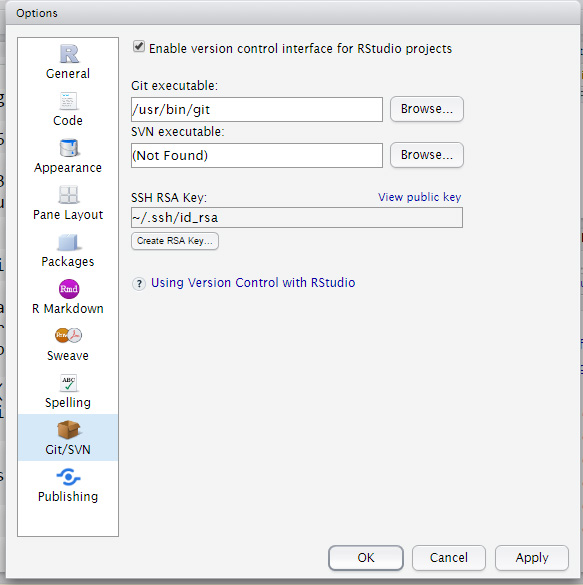
\includegraphics[width=0.5\textwidth]{graphics/CreatingSSH.jpg}
\caption{After natigating through the Rstudio Git/SNV menu, select `Create an RSA Key'.}
\end{figure}

\NP You have the option to create a passphrase. I suggest you don't to make it easier for now. But should your have projects that need extra security, this is a good idea.

\NP After you hit the ``Create'' button an image will be generated in a pop-up window -- As far as I can tell, this image is some sort of encryption thing -- but I don't see any reason why we should care. So, close this pop-up window. 

\NP Next, select the `View the public key' and copy the contents of the pop-up window using cntrl-c. Now we need to paste that key into Github. NOTE: If you closed all the windows, you have to nagivate back to the Git/SVN menu via Global Options. 

\NP Add RSA/SSH Key to Github
  \begin{enumerate}
  \item Go to Profile, in the upper right top of the Github page. Unless you have uploaded a picture of yourself, profile image is a tetris looking icon.
  \item Select the menu item ``Settings.''
  \item Using the left menu, select the ``SSH and GPG keys'' button.
  \item Click on new SSH key, type in name of key (e.g. 'myRstudio SSH key')
  
\begin{figure}
\centering
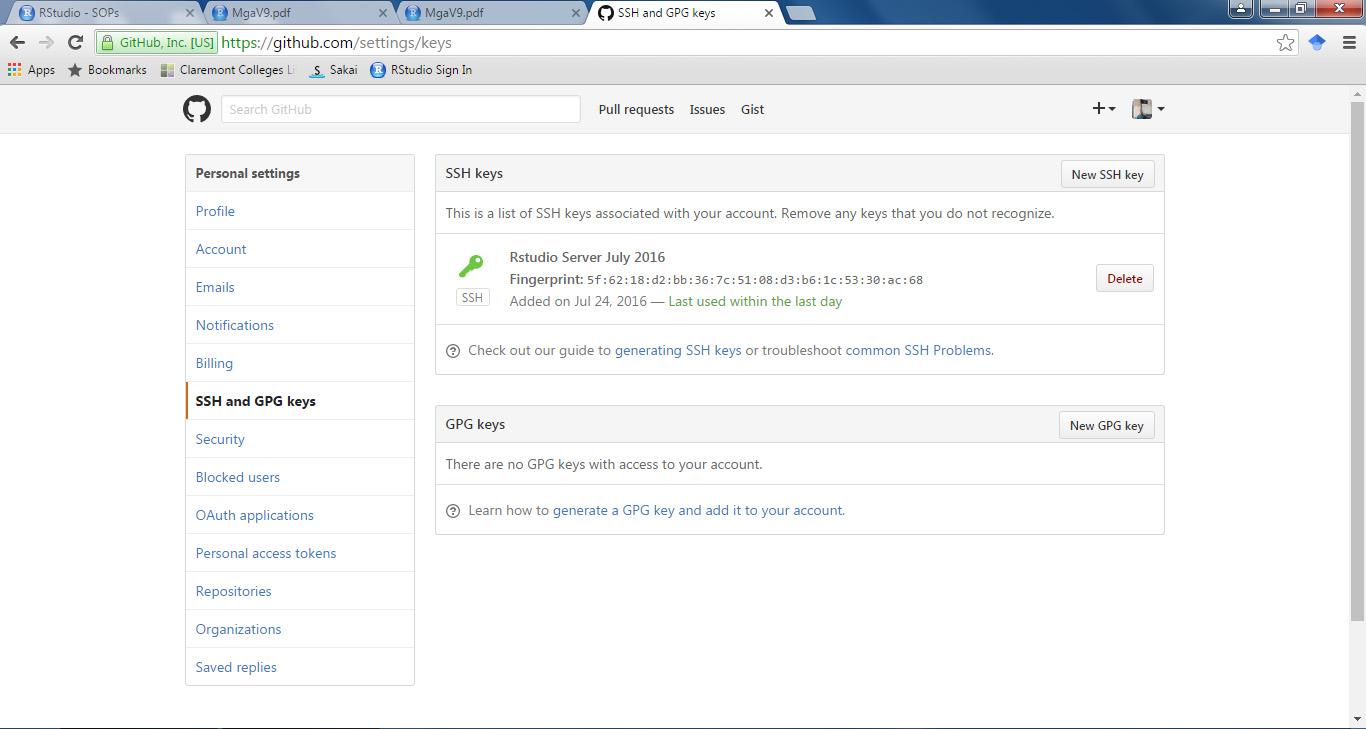
\includegraphics[width=0.8\textwidth]{graphics/Github_SavedSSH.jpg}
\caption{Creating the connection between Rstudio and Gitub requires a `key'. We generate the key in Rstudio and then we tell Github what the key is.}
\end{figure}

  \item Paste in the RSA key, from your clipboard, into the window below.
  \item Hit green ``add SSH key'' button.
  \item Github and R can now communicate.
  \end{enumerate}


\subsection{Linking an RStudio Project to a Github Repository}

\NP To link a Github respository in Rstudio, you will need to ``clone'' the site, while we create a new project in R studio.


\begin{figure}[H]
\centering
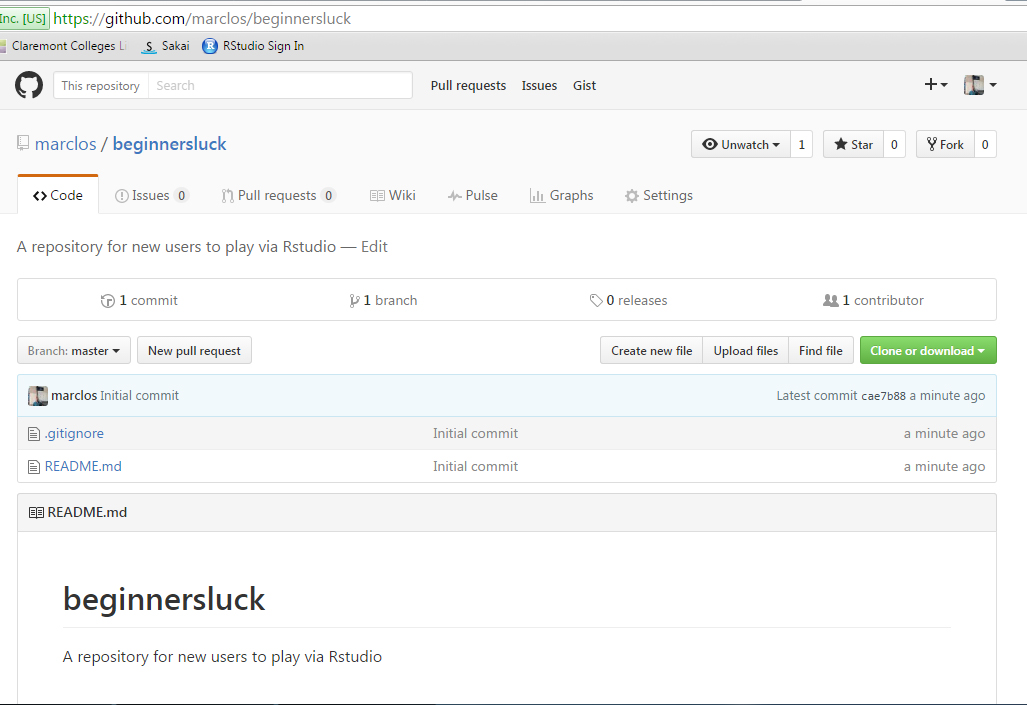
\includegraphics[width=0.8\textwidth]{graphics/CloningGithub.jpg}
\caption{Step 1: Select the green button, "Clone or Download"}
\label{fig:step1}
\end{figure}

\NP I have created a simple repository to begin learning how to use R Studio.

\NP Search Github for the following repository name, 'beginnersluck'. There are several, so you'll have to find the one I created, under the username, 'marclos'. 

\NP Select this repository. Note the 'README.md', click on it to view it. The suffix, md, referrs to markdown, which is a simple languague for things to display on the web.

\NP We need to get the url and SSH key for Rstudio and to accomplish this we ``Clone'' the Github repository. Click on the ''clone or download'' button (Figure \ref{fig:step1}).


\NP Next we will 'Clone with SSH'. If the header says 'Clone with HTTPS', you can toggle the selection with the small 'Use SSH' link in the upper right of the box. If you skip switching to SSH, it's really hard to fix the project afterwards. You can copy the clone information by clicking on the little clipboard on the right of the address (Figure \ref{fig:step2}).

\begin{figure}[H]
\centering
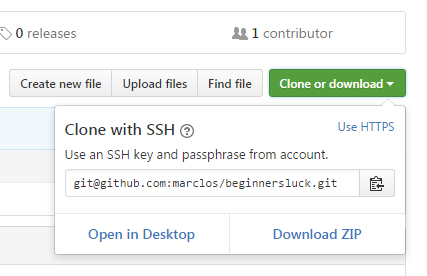
\includegraphics[width=0.5\textwidth]{graphics/CloningGithub2.jpg}
\caption{Step 2: Be sure you clone with SSH!}
\label{fig:step2}
\end{figure}

\NP Now we return to Rstudio and create a new project. Navigate to the file toolbar and select ``New Project''. Where you will be greeted with three choices (Figure \ref{fig:step3}). Select 'Version Control'. 
\begin{figure}[H]
\centering
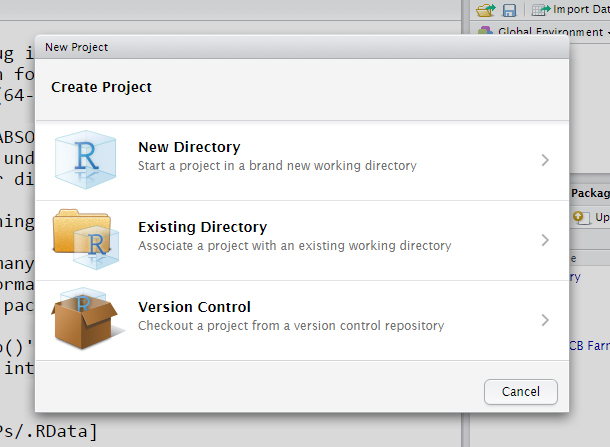
\includegraphics[width=0.5\textwidth]{graphics/RstudioNewProject.jpg}
\caption{Step 3: When you create a new project, you have three choices. Select 'Version Control' to clone your repository.}
\label{fig:step3}
\end{figure}

\NP Once you have selected the Version Control, you have one more choice to make, luckily this is pretty easy, select ``Git'' (Figure \ref{fig:step4}).

\begin{figure}[H]
\centering
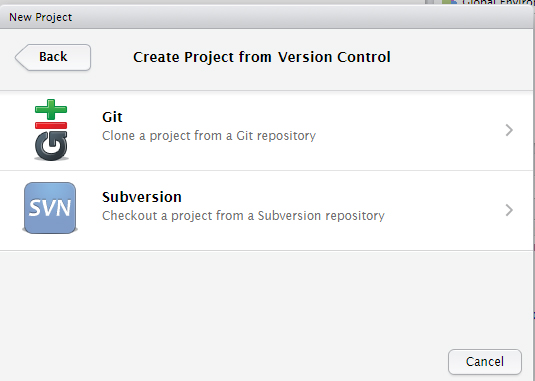
\includegraphics[width=0.5\textwidth]{graphics/RstudioNewProject2.jpg}
\caption{Step 4: Select ``Git'' to clone the repository.}
\label{fig:step4}
\end{figure}

When you arrive in the ``Clone Git Repostory'' window, you can simply paste your clipboard into the Repository URL. This usually fills in the project directory name too. But if not, you can type in the name, in this case, "beginnersluck" (Figure \ref{fig:step5}).

\begin{figure}[H]
\centering
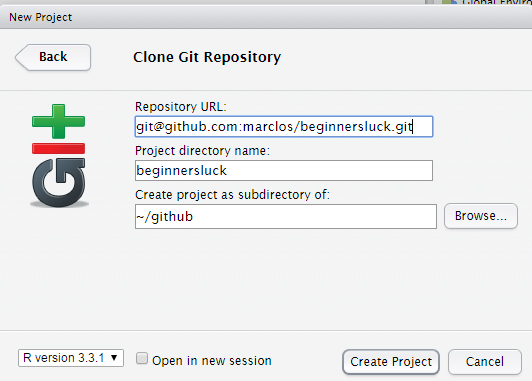
\includegraphics[width=0.5\textwidth]{graphics/RstudioNewProject3.jpg}
\caption{Step 5: You should have something useful in each of the boxes.}
\label{fig:step5}
\end{figure}

\NP For many new users, Rstudio may claim some problem establishing authenticity (Figure \ref{fig:step6}). Type 'yes'. Then hit okay. I am not exactly sure why this step exists. 

\begin{figure}[H]
\centering
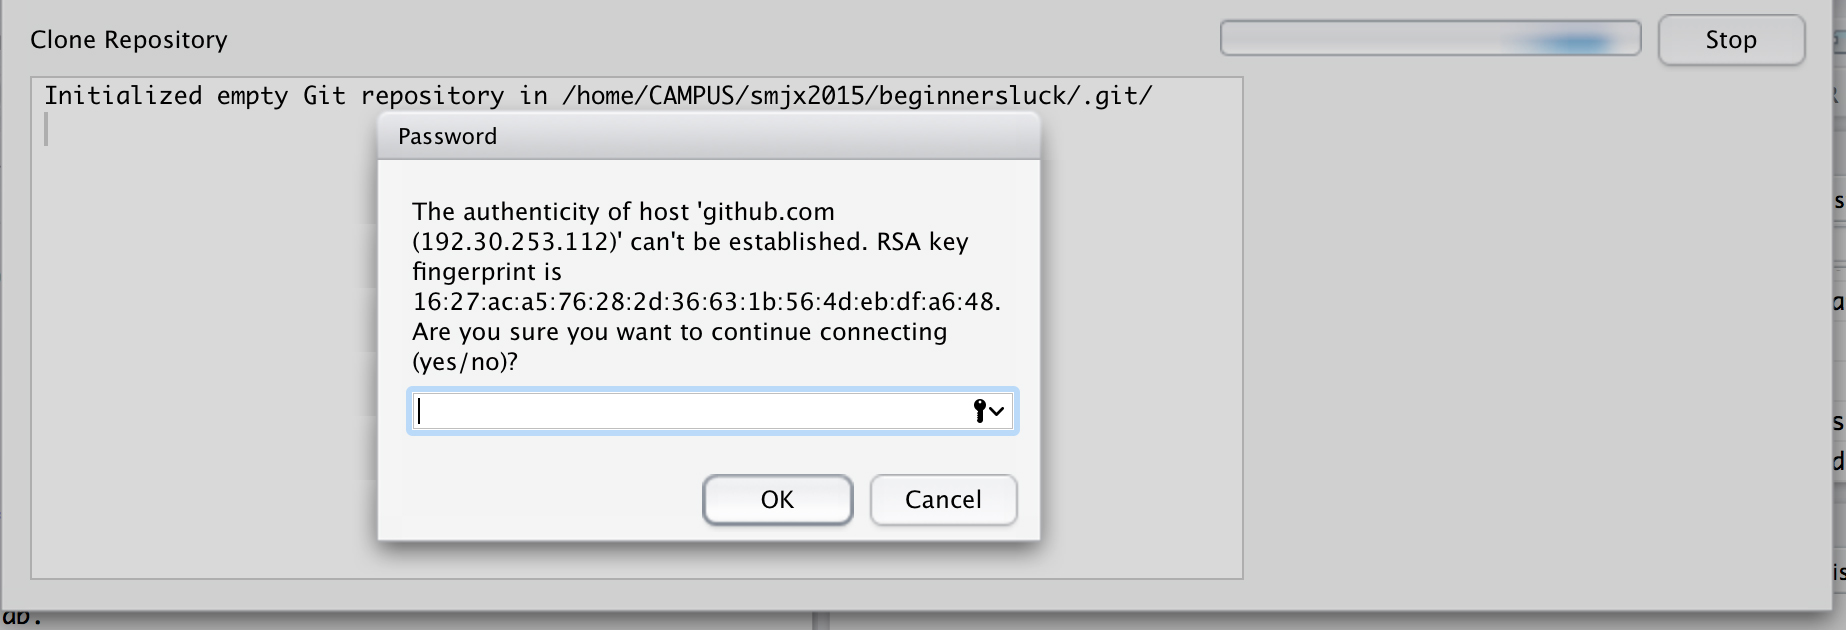
\includegraphics[width=0.99\textwidth]{graphics/Authenticity.jpg}
\caption{Step 6: You should have something useful in each of the boxes.}
\label{fig:step6}
\end{figure}


\NP Now you should see a few files from the repository on your Rstudio window. Open them up and see what they are to get familiar with them.

\NP If nothing comes up, your pop-up blocker is activated. Turn off the pop-up blocker for this site and try again. 

\NP The easiest place to begin, is to `Pull' a repository once you have cloned it. 

\NP Any user can pull public repsitories. 

\NP Everytime you want to use something from a respository you want to pull to get the most up-to-date versions. 

\NP Now that you have created connectivity you can create your own repository. But first you need to create a project in Rstudio. I suggest you the following steps as you begin:


\subsection{Pulling a Repository}

\NP Pulling a Repository is downloading all the changed files into your local (or server) directory. Using the downward facing blue arrow that labeled ``Pull'' in the Git tab in Rstudio.

\section{Becoming a Collaborator}

\NP To contribute to a project, you must be able ``Push'' and ``Pull'' to the respository. 

\NP When you are working on someone else's repository they will need to add you as a collaborator. And to accomplish this, it is easiest to send your user name to the owner, so she can add you to the collaborator list.  

\NP Once this has been done you can ``Push'' and ``Pull'' to the respository, but let's learn more about how to use R to create this project. 




\section{Working on Projects in Rstudio}


\section{Downloading R, Rstudio, and Github as desktop programs}

\NP Note new users: Please use the server mode to begin using this software. Later you can use the desktop versions. 

\NP To accomplish install the programs on the local harddrive, download and install the programs in the following order: 

\begin{enumerate}
  \item R \url{https://cran.r-project.org/}
  \item RStudio \url{https://www.rstudio.com/}
  \item Github desktop \url{https://desktop.github.com/}
\end{enumerate}


\subsection{Best Practices}

\begin{description}
  \item[Pull] When you open RStudio, the first thing you should do is ``Pull'' from the repository to ensure your files are up-to-date. When you "Pull", you will get one of three results:
  
  \begin{description}
  \item[Already up-to-date.] This means that your files have not been updated on the Github site since you last pulled the files. If you suspect someone has worked on the files, but are not getting those changes, it means that your collaborator has failed to ``Push'' these changes onto the repsository. If this is the case, you might need to go to the troubleshooting question to address this problem.
  
  \item[Successful Updates] If your files are successfully updated from the repository, you will see:
  
summary of updates

master 6038765 Started to explain set up procedures
 
 5 files changed, 434 insertions(+), 8 deletions(-)
 
 create mode 100644 06\_Rstudio\_Github/Rstudio-and-Github-concordance.tex
 
 create mode 100644 06\_Rstudio\_Github/Rstudio-and-Github.log
 
 create mode 100644 06\_Rstudio\_Github/Rstudio-and-Github.pdf
 
 create mode 100644 06\_Rstudio\_Github/Rstudio-and-Github.tex
 
 \item[Unsuccesful "Pull"]
 
 
\end{description}

  \item[Commit]
  \item[Push] As you might guess, when you ``Push'' you can also have several outcomes:
\begin{description}
  \item[Everything up-to-date] is certainly simple.   \item[Successful ``Push'']
  
    "To git@github.com:marclos/SOPs.git
  
   e2efe6f..0b18250  master -> master"
   \item[Unsuccessful "Push"]
\end{description}
  
  
Basically git commit ``records changes to the repository'' while git push ``updates remote refs along with associated objects''. So the first one is used in connection with your local repository, while the latter one is used to interact with a remote repository.

Here is a nice picture from Oliver Steele, that explains the git model and the commands:  

\begin{figure}
\centering
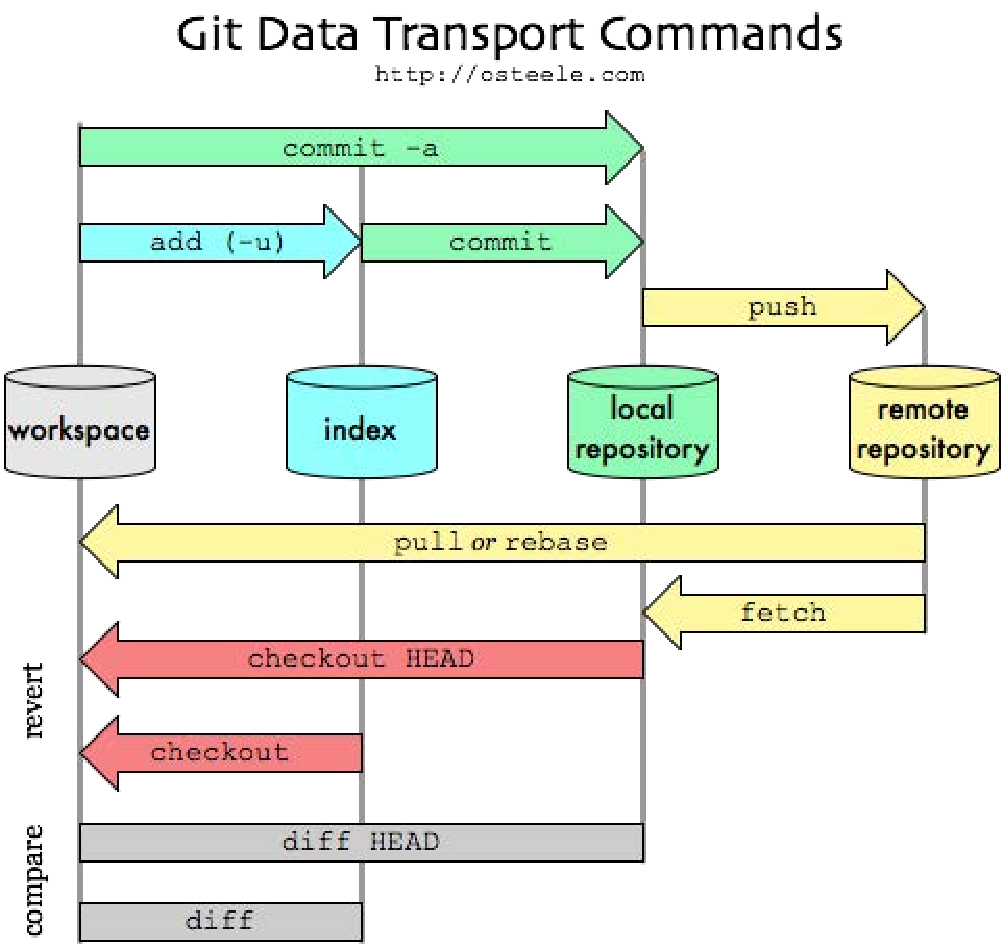
\includegraphics[width=0.5\textwidth]{graphics/MgaV9}
\end{figure}
   
\end{description}

\section{Creating a shared R Project}

\NP Learning to create a shared R project will help you create an understanding of the work flow, where we 

\begin{enumerate}
\item Create a New Repository (if necessary)
\item Clone the respository
\item Pull 
\item create a test file
\item Push
\end{enumerate}

\NP At this point, you can start using the Github respitories that have already been created.

\subsection{Creating a New Repository}

\NP Creating a respository in Github is pretty easy, but there are a couple of decision points worth pointing out.

\NP Click on the green ``New Repository'' button.

\NP A new page comes up and provides space for the name of the new repository. If you leave spaces, Github will automatically insert dashes between the words.

\NP Decide if you want the site to be public or private. NOTE: Usually to get a private site, you have to pay, however, you can apply for an academic account where you can have private accounts. 

\NP Check the box if you want a README.md file created. I always create one -- you can do it later, but it's nice to document what you are doing, so I suggest you create one.

\NP Some files are not worth push and pulling all the time, but these files depend on the program you are using. In this case, we can have github ignore all files that are associated with R that don't really contribute to the project itself. So, I suggest you add these files to the .ignore file. You can add these later too, but it's a bit tricker.

\NP Finally, Github allows you to create a licence to protect your work. I need to do some research about the differences, but I usually pick 'GNU General Public Licence' for no good reason, besides it sounds good.

\NP The respository is now created, but Rstudio doesn't have access to it yet. You'll need to pull the respistory.

\subsection{Clone New Project}

\subsection{Create and knitr new Rmd file}

\subsection{Commit changes}

\subsection{Push}

\section{Troubleshooting}

\subsection {Identity Error}

\NP An identity error is... 

\begin{figure}[H]
\centering
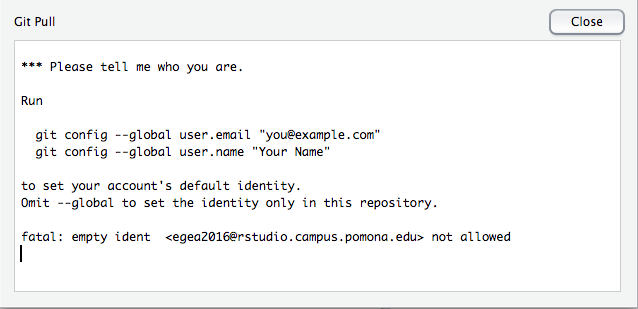
\includegraphics[width=0.5\textwidth]{graphics/IdentityError.png}
\caption{Enter email and name}
\end{figure}

\NP If you recieve an error as shown in the figure above, we can fix this using the Git shell. IN the ``Git'' tab, click on the gear icon and select ``Shell...'' 

\NP A new window will be shown and then type after the prompt:

'git config ...
'git config... '

\NP These commands should sync rstudio to Github based on your email and name.


\subsection{Push, Pull, and Merge Errors}

\NP At first when you're a newcomer to working on projects within Rstudio connected to a GitHub repository, you may forget the ``best practices`` of pulling, committing and pushing described above. You might have already gone through all the steps involved in setting up your GitHub account, linking your workspace in Rstudio with the correct project, and begun work on a specific file, but if you forget to update your workspace each time you come back to modify a file (especially in the case of coming back the next day to a file in Rstudio and forgetting to pull changes other collaborators may have made), you will run into problems committing, and pushing your changes. In this most common case, it's not likely that you'll notice any problems until you try to commit your changes. Thus, we'll begin this section on trouble shooting problems with Github and Rstudio at the committ level.

\NP Alternatively, if you and others edit the same section, Github is going to need some ``human'' decision making to negotiate these changes. In Github jargon, this requires one to 'merge' changes. 
\NP (un)Fortunately, students are very good at discovering ways that the pull/commit/push process can be disrupted. As each case comes to my attention, I ask for a screen shot and a description, so we can trouble shoot each problem when they present themselves.

\subsection{`Commit' Problems}
\NP In the scenario described above, you will get an error code when trying to committ your new changes to a file. 

\subsection{`Merge' Errors}

\NP If you find merge errors it often means that you and someone else has modified a file and they need to be reconciled.

\begin{figure}
\centering
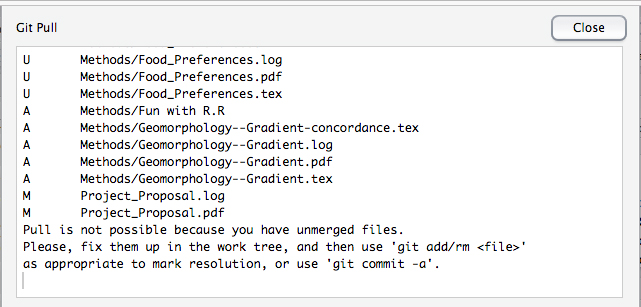
\includegraphics[width=0.5\textwidth]{graphics/UnmergedError.jpg}
\end{figure}

\NP Before trying to commit changes, We need to merge changes in the work tree. 

\NP To do this go to the list in the upper right hand corner of workspace in Rstudio studio (select the Git tab). In this list you should see your file changes, as well as other changes. 

\NP Select the files that have blue squares with your initials. The important part is to find the places where there is a multiple squares (ie. Blue squares, orange squares and red squares). Multiple squares signify that those sections there were changes made to the file that over lap and there should be a U next to the checkbox on those lines. Click those checkboxes. 

\NP Then commit and push changes. 

\begin{figure}
\centering
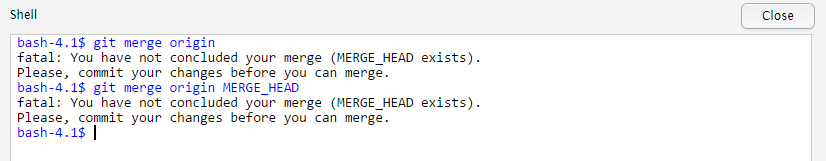
\includegraphics[width=0.5\textwidth]{graphics/MergeError.jpg}
\end{figure}

\subsection{`Pull' is rejected}

\NP Merging changes... how??

Pull is not possible because you have unmerged files.
Please, fix them up in the work tree, and then use 'git add/rm <file>'
as appropriate to mark resolution, or use 'git commit -a'.

Ideally, if one gets a merge conflict, he should resolve them manually, and commit the changes using git add file.name \&\& git commit -m '''removed merge conflicts''. Now, another user has updated the files in question on his repository, and has pushed his changes to the common upstream repo.

It so happens, that your merge conflicts from (probably) the last commit were not not resolved, so your files are not merged all right, and hence the U(unmerged) flag for the files. So now, when you do a git pull, git is throwing up the error, because you have some version of the file, which is not correctly resolved.

To resolve this, you will have to resolve the merge conflicts in question, and add and commit the changes, before you can do a git pull.

\subsection{Dealing with non-fast-forward errors}

\NP Sometimes, Git can't make your change to a remote repository without losing commits. When this happens, your push is refused. If another person has pushed to the same branch as you, Git won't be able to push your changes.

\NP You can fix this by fetching and merging the changes made on the remote branch with the changes that you have made locally:
\begin{itemize}
  \item \$ git fetch origin
  \item \# Fetches updates made to an online repository
  \item \$ git merge origin YOUR\_BRANCH\_NAME
  \item \# Merges updates made online with your local work
\end{itemize}

\NP Or, you can simply use git pull to perform both commands at once.



\subsection{`Push` fails}

\NP Below are several potential remedies:

\begin{description}
  \item[merge] asdfasdf
  
  \item[Deleting a Project in R Studio]If you are willing to sacrifice the changes you made or have mailed them to a collaborator to deal with you can delete the entire project in Rstudio. To accomplish this delete all files in directory, clear workspace and console, don't save, then go to session tab: Terminate R, and hopefully that will do the trick. Then commence with starting a new project. 

\end{description}

%\section{Data Analysis and Calculations}

%\section{QC/QA Criteria}

\section{Collaboration and Version Control}

\subsection{Adding Collaborators}
\NP Go to Profile, repository, toolbar in repository click settings, click on collaboration. Add usernames of collaborators to give them permission to collab.

\subsection{Workflow tracking}

\NP Collaborators can create ways that each one is responsible for certain activities..

\NP Branching...
 

\section{References}

\NP 





\end{document}
